\documentclass[11pt]{article}
\usepackage{../EllioStyle}
\usepackage{listings}

\definecolor{codegreen}{rgb}{0,0.6,0}
\definecolor{codegray}{rgb}{0.5,0.5,0.5}
\definecolor{codepurple}{rgb}{0.58,0,0.82}
\definecolor{backcolour}{rgb}{0.95,0.95,0.92}

\graphicspath{ {imgs/} }

\title{Homework 1}
\author{Elliott Pryor}
\date{30 September 2023}

\rhead{Homework 1}

\begin{document}
\maketitle

My work can be found on my github:
\href{https://github.com/ElliottP-13/DeepRL-Course/tree/main/hw1}{https://github.com/ElliottP-13/DeepRL-Course}.


\problem{1}

Consider the problem of imitation learning within a discrete MDP with horizon $T$ and an expert
policy $\pi^*$. We gather expert demonstrations from $\pi^*$ and fit an imitation policy $\pi_\theta$ to these
trajectories so that

\begin{equation}
    \mathbb{E}_{p_{\pi^*}(s)} \pi_\theta(a \neq \pi^*(s)) = \frac{1}{T} \sum^{T}_{t=1} \mathbb{E}_{p_{\pi^*}(s_t)} \pi_\theta(a \neq \pi^*(s_t)) \leq \epsilon
\end{equation}
i.e., the expected likelihood that the learned policy $\pi_\theta$ disagrees with the expert $\pi^*$ within the
training distribution $p_{\pi^*}$ of states drawn from random expert trajectories is at most $\epsilon$.
For convenience, the notation $p_\pi (s_t)$ indicates the state distribution under $\pi$ at time step $t$ while
$p(s)$ indicates the state marginal of $\pi$ across time steps, unless indicated otherwise

\begin{enumerate}
    \item Show that $\sum_{s_t} \left| p_{\pi_\theta}(st) - p_{\pi^*}(st) \right| \leq 2T\epsilon$
    \item Consider the expected return of the learned policy $\pi_\theta$ for a state-dependent reward function $r(s_t)$.
    where we assume the reward is bounded $|r(s_t)| \leq R_{max}$:
    $$
    J(\pi) = \sum_{t=1}^T \mathbb{E}_{p_\pi(s_t)} r(s_t)
    $$
        \begin{enumerate}
            \item Show that $|J(\pi_\theta) - J(\pi^*)| \in \mathcal{O}(T\epsilon)$ when the reward only depends on the last state.
            I.e., $r(s_t) = 0$ $\forall t<T$
            \item Show that $J(\pi*) - J(\pi_\theta) \in \mathcal{O}(T^2 \epsilon)$
        \end{enumerate}
\end{enumerate}

\soln

\begin{enumerate}
    \item So we want to show that $\sum_{s_t} \left| p_{\pi_\theta}(st) - p_{\pi^*}(st) \right| \leq 2T\epsilon$.
    We know that $\mathbb{E}_{p_{\pi^*}(s)} \pi_\theta(a \neq \pi^*(s)) = \frac{1}{T} \sum^{T}_{t=1} \mathbb{E}_{p_{\pi^*}(s_t)} \pi_\theta(a \neq \pi^*(s_t)) \leq \epsilon$.
    This means that the expected value of the probability that $\pi_\theta$ disagrees with $\pi^*$ is at most $\epsilon$.
    
    We note that if there is no mistake, then there is no difference in the state distribution. 
    In the worst case, after a mistake the state distribution is completely different, so $\left| p_{\pi_\theta}(st) - p_{\pi^*}(st) \right| = 2 \; \forall t>t_{mistake}$.
    Thus the cost after the mistake would be: $2(T - t_{mistake})$.
    We partition the space by the time of the mistake:
    $\epsilon * cost_1 , (1-\epsilon)\epsilon * cost_2 , (1-\epsilon)^2\epsilon *cost_3 , \dots , (1 - \epsilon)^T * 0$.
    Where cost is the total difference in the state distribution after the mistake.
    So all the possible costs that we can incur are: $\epsilon * 2T , (1-\epsilon)\epsilon * 2(T-1) , (1-\epsilon)^2\epsilon *2(T-2) , \dots , (1 - \epsilon)^T * 0$.
    So the worst case is we make a mistake on the very first sample.
    Thus $\sum_{s_t} \left| p_{\pi_\theta}(st) - p_{\pi^*}(st) \right| \leq 2T\epsilon$

    \item \begin{enumerate}
        \item We want to show that $|J(\pi_\theta) - J(\pi^*)| \in \mathcal{O}(T\epsilon)$ when the reward only depends on the last state.
        This bound is somewhat misleading as it appears to grow linearly, but in fact is constant. 
        This is because the reward only depends on the last state, so $|J(\pi_\theta) - J(\pi^*)| = |\mathbb{E}_{p_{\pi^*}(s_T)}(r(s_T)) - \mathbb{E}_{p_{\pi_\theta}(s_T)}(r(s_T))|$.
        We know that $r(s)$ is a bounded function, so this is clearly $\leq R_{max}$ which is constant.

        We can also derive the original (linear) bound fairly easily. We partition it into the case of no mistakes and the case of mistakes.
        No mistake occurs with probability $(1-\epsilon)^T$ which by Bernoulli's inequality is $\geq 1 - T\epsilon$.
        This means the probability of a mistake is $\leq 1 - (1 - T\epsilon) = T\epsilon$. We can assume worst case cost if a mistake occurs.
        Thus the expected value of the cost $\leq (1 - T \epsilon) *0 + (T\epsilon)*R_{max} \in \mathcal{T\epsilon}$

        \item Given the previous result, we consider the generic case where the reward depends on all states, as a sum of cases where the reward only depends on the last state.
        Let $j(T)$ denote the cost discovered in the previous section $j(t) = t \epsilon * R_{max}$.  Then the generic case:
        \begin{align*}
            |J(\pi*) - J(\pi_\theta)| &\leq j(1) + j(2) + \dots + j(T)\\
            &= \epsilon * R_{max} * (1 + 2 + \dots + T)\\
            &= \epsilon * R_{max} * \frac{T(T+1)}{2}\\
            &= \epsilon * R_{max} * \left(\frac{T^2}{2} + \frac{T}{2} \right)\\
            &\in \mathcal{O}(T^2 \epsilon)    
        \end{align*}
    \end{enumerate}
    
\end{enumerate}

\problem{2}

Run behavioral cloning (BC) and report results on two tasks: the Ant environment, where
a behavioral cloning agent should achieve at least 30\% of the performance of the expert, and
one environment of your choosing where it does not.
\soln

Figure \ref{fig:ant} show the results on the ant environment with default hyperparameters.
2 layers, of 64 nodes, 0.005 lr, batch size = 1000, train steps = 1000. Metrics were computed over 5 rollouts (Eval batch size = 5000, ep len = 1000).

\begin{figure}[h]
    \centering
    \begin{subfigure}[b]{0.47\textwidth}
        \centering
        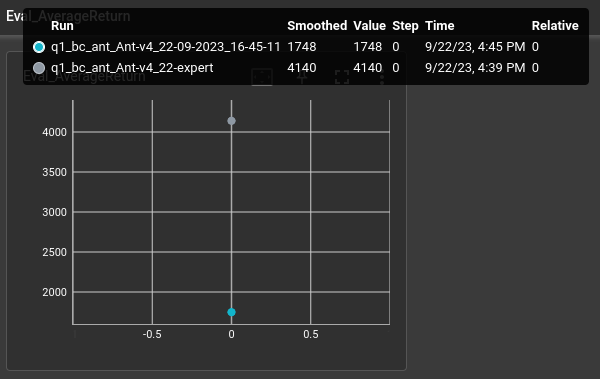
\includegraphics[width=\textwidth]{09-22-ant_mean}
        \caption{Mean Returns}
        \label{fig:ant_mean}
    \end{subfigure}
    \hfill
    \begin{subfigure}[b]{0.47\textwidth}
        \centering
        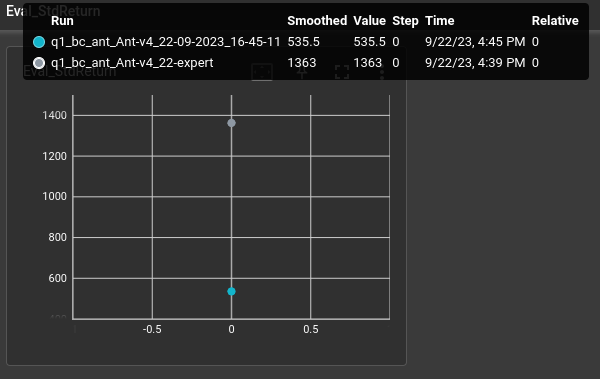
\includegraphics[width=\textwidth]{09-22-ant_std}
        \caption{Std of Returns}
        \label{fig:ant_std}
    \end{subfigure}
    \caption{Ant environment with 5 repeats (eval batch size = 5000, batch size = 1000). Blue is expert, grey is BC.}
    \label{fig:ant}
\end{figure}

Figure \ref{fig:hop} show the results on the hopper environment with default hyperparameters.
We see much worse performance here, indicating that the BC agent did not work as well.
This could be because the environment is much more challenging, and possibly a larger network would be needed.
\begin{figure}[h]
    \centering
    \begin{subfigure}[b]{0.47\textwidth}
        \centering
        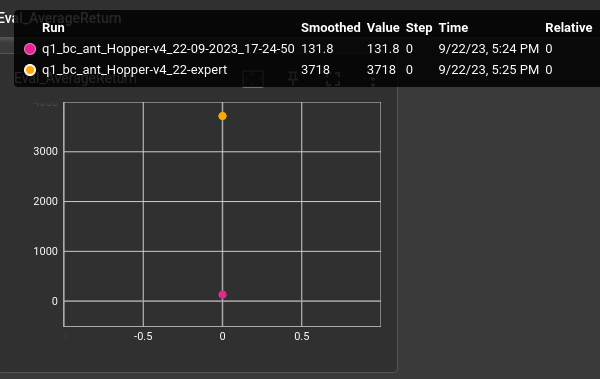
\includegraphics[width=\textwidth]{09-22-hop_mean}
        \caption{Mean Returns}
        \label{fig:hop_mean}
    \end{subfigure}
    \hfill
    \begin{subfigure}[b]{0.47\textwidth}
        \centering
        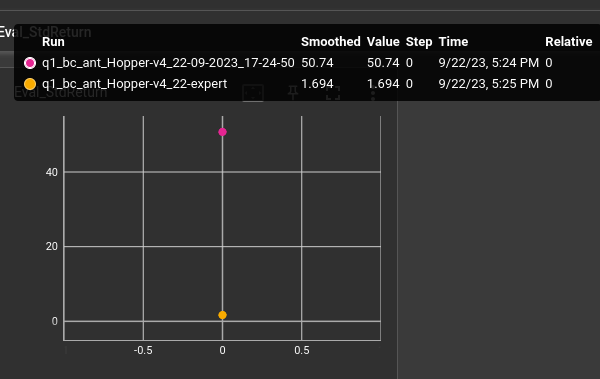
\includegraphics[width=\textwidth]{09-22-hop_std}
        \caption{Std of Returns}
        \label{fig:hop_std}
    \end{subfigure}
    \caption{Hopper environment with 5 repeats (eval batch size = 5000, batch size = 1000). Yellow is expert, Pink is BC.}
    \label{fig:hop}
\end{figure}

We try double the network depth in case the network is not large enough to capture the function, 
and 5 times the batch size in order to give it more training data (we also proportionally increase the training iterations), and see the results in Figure \ref{fig:hop2}.
They did not improve the performance, and in fact made it worse.

\begin{figure}[h] 
    \centering
    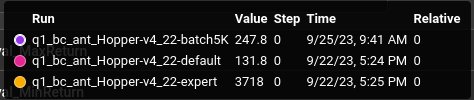
\includegraphics[width=0.55 \linewidth]{09-25-hop_all}
    \caption{Different networks on hopper. This is the mean returns}
    \label{fig:hop2}
\end{figure}

Based on this, we vary batch size more. 
The results can be seen in figure \ref{fig:hop_batch}, the effect is not very significant, and we do not recover 30\% of the expert performance.
\begin{figure}[h!] 
    \centering
    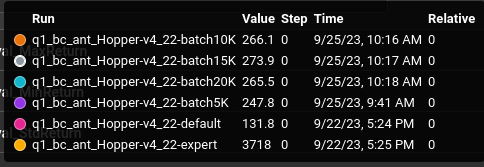
\includegraphics[width=0.55 \linewidth]{09-25-hop_batch}
    \caption{Variation of batch size and training iterations (batch = train) on hopper. This is the mean returns.}
    \label{fig:hop_batch}
\end{figure}

\problem{3}
Run DAgger and report results on the two tasks you tested previously with behavioral cloning
(i.e., Ant + another environment). 

\soln

Figure \ref{fig:ant_dag} show the results on the ant environment with default hyperparameters.
2 layers, of 64 nodes, 0.005 lr. Batch size = 1000, and 10 dagger iterations. Metrics were computed over 5 rollouts.


\begin{figure}[h]
    \centering
    \begin{subfigure}[b]{0.47\textwidth}
        \centering
        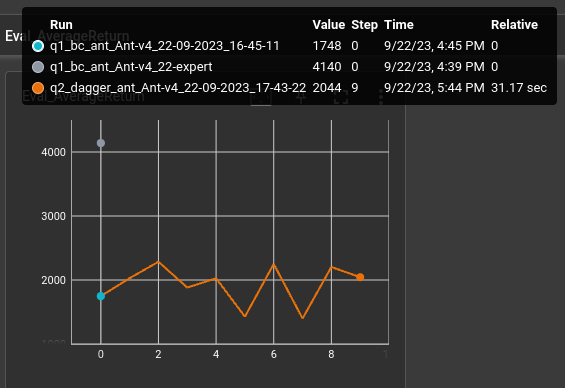
\includegraphics[width=\textwidth]{09-22-dag_ant_mean}
        \caption{Mean Returns}
        \label{fig:ant_mean}
    \end{subfigure}
    \hfill
    \begin{subfigure}[b]{0.47\textwidth}
        \centering
        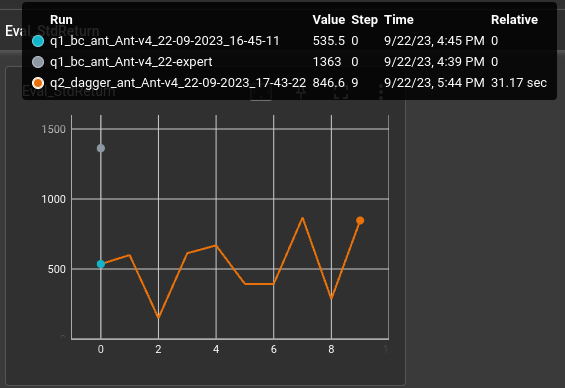
\includegraphics[width=\textwidth]{09-22-dag_ant_std}
        \caption{Std of Returns}
        \label{fig:ant_std}
    \end{subfigure}
    \caption{Ant environment with 5 repeats (eval batch size = 5000, batch size = 1000). Blue is expert, grey is BC, orange is DAgger.}
    \label{fig:ant_dag}
\end{figure}

This result is confusing because it doesn't seem to improve over time.
However, the training loss does decrease (see Figure \ref{fig:loss}), so we are successfully learning more, but this does not help us during eval. 

\begin{figure}[h] 
    \centering
    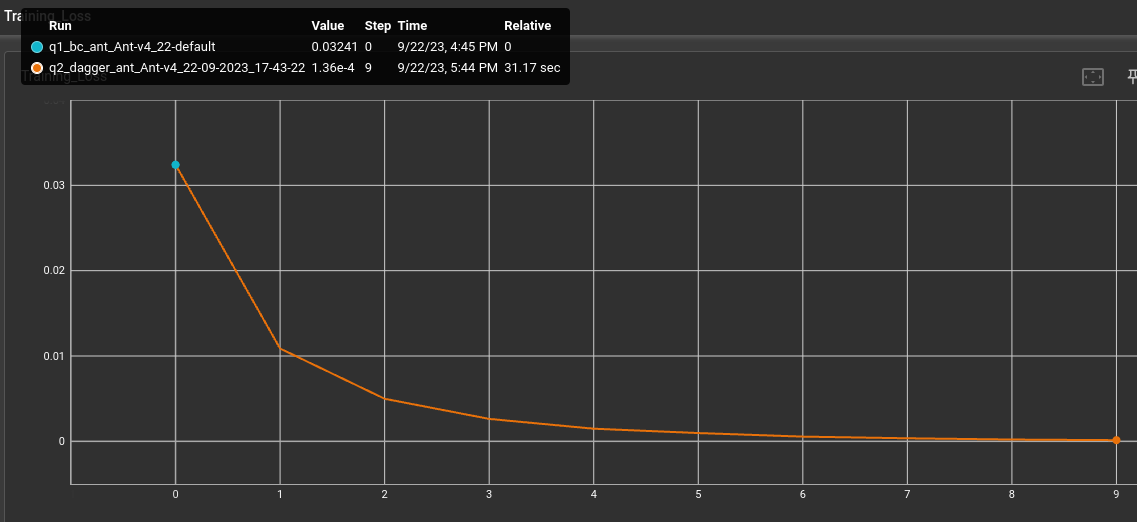
\includegraphics[width=0.55 \linewidth]{09-29-loss}
    \caption{Training loss of Dagger over time}
    \label{fig:loss}
\end{figure}

\begin{figure}[h]
    \centering
    \begin{subfigure}[b]{0.47\textwidth}
        \centering
        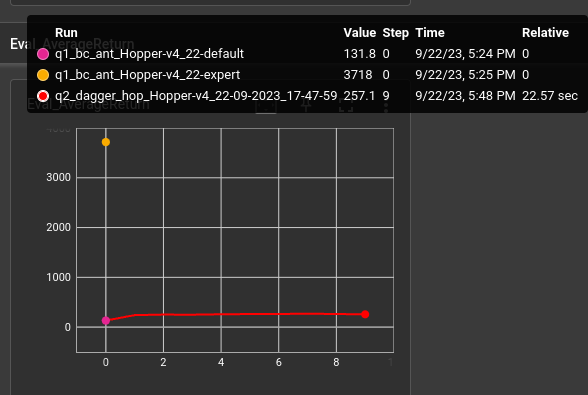
\includegraphics[width=\textwidth]{09-22-dag_hop_mean}
        \caption{Mean Returns}
        \label{fig:hop_mean}
    \end{subfigure}
    \hfill
    \begin{subfigure}[b]{0.47\textwidth}
        \centering
        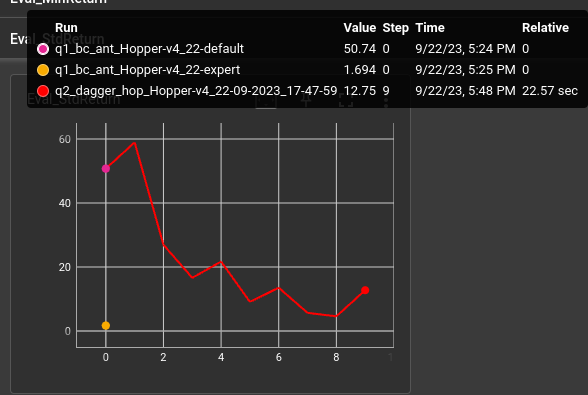
\includegraphics[width=\textwidth]{09-22-dag_hop_std}
        \caption{Std of Returns}
        \label{fig:hop_std}
    \end{subfigure}
    \caption{hop environment with 5 repeats (eval batch size = 5000, batch size = 1000). Yellow is expert, Pink is BC, Red is DAgger.}
    \label{fig:hop_dag}
\end{figure}

We also tried doubling the network depth. And the average returns can be seen in Figure \ref{fig:hop_dag2}.
Once again, the larger network does not seem to do any better.

\begin{figure}[h] 
    \centering
    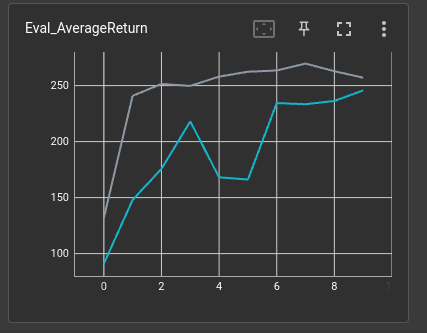
\includegraphics[width=0.55 \linewidth]{09-22-dag_hop_all}
    \caption{Comparison of dagger with defaout network size (grey) and double network depth (blue) in average return.}
    \label{fig:hop_dag2}
\end{figure}

\end{document}